\subsection{Netzwerkprotokolle}
Netzwerkprotokolle besitzen je nach Zweck und Netzwerkschicht verschieden Merkmale und Funktionen. Viele Netzwerkprotokolle hängen von der obersten Schicht bis zur Untersten einen eigenen Protokoll Header an. Dieser besitzt wichtige Merkmale zum Transport der darauf folgenden Daten. Einige der wichtigsten Protokolle und deren Header Funktionen werden in diesem Kapitel genauer betrachtet:\\
\\
\begin{itemize}
\item IP: Das Internet Protocol ist ein sehr weit verbreitetes Netzwerkprotokolle welches die Grundlagen des Internet darstellt. Es befindet sich in der Vermittlungsschicht des OSI-Schichtenmodells und ist somit für die Vermittlung über IP-Adressen zuständig.  
\item TCP: Das Transmission Control Protocol ist ein Netzwerkprotokoll der Transportschicht. Dieses garantiert eine zuverlässige, verbindungsorientierte Transport von Paketen in Computernetzwerken. Es zählt wie das IP-Protokoll zu den Grundlagen des Internets. In diesem Protokoll-Header werden der Quell und Ziel Port genannt, um dem meist zuvor erstellten IP-Paket einen bestimmten Dienst zuzuweisen. Eine TCP-Verbindung erfolgt immer über eine vorgegebene Startsequenz. Diese wird 3-Way-Handshake genannt und wir in Abb. \ref{3way} dargestellt. Dabei werden die Control-Flag-Bits im Header jeweils geändert. 

\begin{figure}[h]
    \centering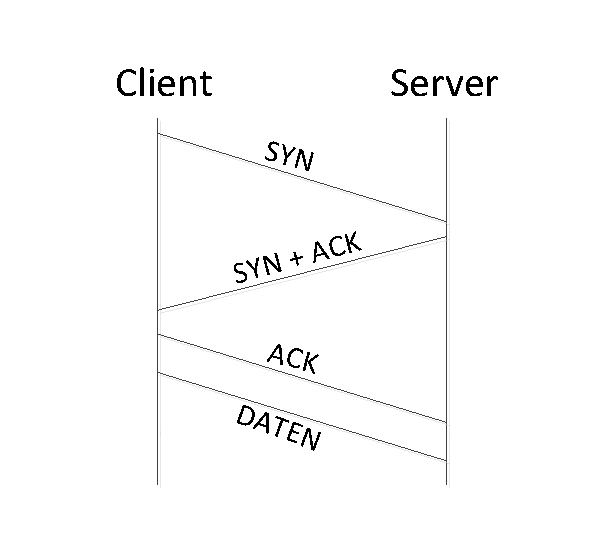
\includegraphics[scale=0.7]{Bilder/3way.pdf}
  \caption{Drei-Wege-Handshake mit TCP}
  \label{3way}
\end{figure}

Nach dem Aufbau der Verbindung können Daten gesendet werden.

\item UDP: Beim User Datagram Protocl handelt es sich um ein verbindungsloses Transportprotokoll. Wie bei TCP befindet sich in seinem Header Ziel- und Quell-Port, jedoch erfolgt kein Verbindungsaufbau. Außerdem wird nicht überprüft, ob alle Pakete tatsächlich beim Benutzer ankommen. 
\item HTTP/HTTPS:Das Hyper Text Transfer Protocol wird von Web-Servern verwendet, um deren Webseiten an den Benutzer zu senden. Diese Protokoll befindet sich bereits in der Anwenderschicht, und baut auf einer TCP/IP Verbindung auf.
\item SSH: Das Secure Shell Protokoll ist ein Netzwerkprotokoll, welches sich ebenfalls auf der Anwenderschicht befindet. Es öffnet eine verschlüsselte Verbindung auf einen entfernten Server, um die Kommandozeile dessen lokal zur Verfügung zu stellen. 
\item FTP: Das File Transfer Protocol wird zur Übertragung von Daten allgemein verwendet. Das Anwendungsprotokoll wird verwendet um vom Server Daten herunter- oder hochzuladen. 
\end{itemize}

\noindent Die Protokolle die in den jeweiligen Schichten angewendet werden, sind oft Angriffsziel vieler Hacker. Diese können über bewusste Manipulation so abgeändert werden, dass das System oft unerwartet reagiert. Einige mögliche Angriffsszenarien werden im folgenden Kapitel betrachtet. 